\documentclass[11pt, oneside]{article}   	% use "amsart" instead of "article" for AMSLaTeX format
\usepackage{geometry}                		% See geometry.pdf to learn the layout options. There are lots.
\geometry{letterpaper}                   	% ... or a4paper or a5paper or ... 
%\geometry{landscape}                		% Activate for rotated page geometry
\usepackage[parfill]{parskip}    	% Activate to begin paragraphs with an empty line rather than an indent
\usepackage{graphicx}				% Use pdf, png, jpg, or eps§ with pdflatex; use eps in DVI mode
								% TeX will automatically convert eps --> pdf in pdflatex		
\usepackage{amssymb}
\usepackage{amsmath}
\usepackage{caption}
%SetFonts

%SetFonts


\title{DL4DS Legal Contract Dataset}
\author{Ethan Chang, Heng Chang, Josh Yip}
\date{April, 2024}		% Activate to display a given date or no date

\begin{document}
\maketitle
\begin{abstract}
	This project aims to develop a high-quality, labeled dataset of legal contract clauses to support AI-driven contract analysis. We introduce a hybrid clause segmentation pipeline that merges regex-based heuristics, semantic similarity using sentence embeddings, and supervised boundary classification to accurately detect clause boundaries in unstructured legal text. Building on this foundation, we assign contract-type-specific clause labels and explore intra-contract relationships by analyzing semantic and structural connections between clauses within the same document. Our work enhances the granularity and contextual understanding of contract language, enabling more robust clause classification, summarization, and fairness analysis.
\end{abstract}

\section*{Introduction}

Legal contracts are complex documents filled with dense, technical language that can be difficult to analyze and understand without expert knowledge. With the growing demand for AI-assisted legal tools, there is a critical need for structured, high-quality datasets that support tasks like clause segmentation, classification, and summarization. Existing legal NLP datasets, such as CUAD and ContractNLI, provide useful foundations, but they often lack fine-grained clause-level annotations and domain-specific context.

Our project addresses this gap by building a dataset and system capable of accurately identifying and labeling contract clauses. We implement a hybrid clause segmentation pipeline that combines regex-based patterns, semantic similarity modeling, and supervised classification to detect clause boundaries with high precision. After segmentation, we apply contract-type-specific clause categorization and explore intra-contract clause relationships to model how clauses interrelate within the same legal context.

This work contributes a reproducible framework for fine-grained contract analysis, with applications in contract review, compliance checking, and legal summarization. Our code and documentation are available at:
https://github.com/joshyipp/542-LegalContract-AI.git.
\section*{Related Work}
Contract analysis has advanced with new datasets and methods for clause segmentation and labeling. One prominent dataset is the \textit{Contract Understanding Atticus Dataset (CUAD)} curated by the Atticus Project. CUAD v1 contains 510 commercial contracts annotated by lawyers with over 13{,}000 clause labels spanning 41 clause types~\cite{hendrycks2021cuad}. Its task is to identify salient contract passages that matter in legal review. As Hendrycks et al.\ note, CUAD’s expert-annotated corpus “consists of over 13,000 annotations” and enables benchmarking of models on legal clause identification.

Stanford’s \textit{ContractNLI} dataset offers a different angle, framing contract analysis as document-level natural language inference~\cite{koreeda2021contractnli}. ContractNLI annotates 607 non-disclosure agreements (NDAs) with entailment, contradiction, or neutral labels for 17 fixed hypotheses. It is described as “the first dataset to utilize NLI for contracts” and, as of 2021, the largest annotated contract corpus. Both CUAD and ContractNLI provide valuable benchmarks, but they differ in scope: CUAD’s clause categories apply broadly to deal contracts, whereas ContractNLI focuses narrowly on NDAs and inference. Other specialized corpora exist (e.g., contracts labeled for rights and obligations), but none has combined clause-level segmentation with contract-type-specific categorization to the extent of our project.

Before the era of large datasets, rule-based approaches often drove clause segmentation. Practical tools---such as e-discovery software like Relativity---exploit document structure: for example, Relativity’s contracts module splits a document into sections by detecting section headings and outline cues~\cite{relativitydocs}. Likewise, custom pipelines frequently apply regular expressions to capture known markers such as “Table of Contents” or numbered section titles. For example, in one insurance-contract processing system, regex is first used to locate and clean the table of contents, and then section titles are matched in the contract body to create paragraph-level segments~\cite{goossens2017processing}. As shown in that study, this approach yields distinct “paragraph 1, paragraph 2…” units.

These methods successfully segment contracts into logical units, but they rely on rigid patterns (e.g., headings, keywords, punctuation) and may fail when contracts exhibit nonstandard formatting. In research literature, similar ideas appear: Chalkidis and Androutsopoulos~\cite{chalkidis2017extraction} essentially carved contracts into fixed “extraction zones” for each clause type. In short, prior work often uses regex or layout rules to hypothesize clause boundaries before any learning occurs.

More recent work has explored machine learning and semantic methods for clause extraction. Many approaches assume segmented text and focus on classification. For example, transformers fine-tuned on CUAD can predict clause labels, though Hendrycks et al.\ note that model performance remains far from perfect. Xu et al.’s \textit{ConReader} (2022) explicitly goes beyond local context by modeling intra-contract relations~\cite{xu2022conreader}. They identify three key clause-level links in contracts---long-range context links, term--definition pairs, and similarity between same-type clauses---and incorporate them to improve clause-level extraction. Similarly, Borchmann et al.~\cite{borchmann2020contract} defined a “contract discovery” task where a model retrieves clauses similar to given examples; their findings showed that off-the-shelf encoders struggle with few-shot clause retrieval.

In all these cases, however, the input clause spans are often assumed to be known or pre-segmented. Few prior works simultaneously address both identifying clause boundaries and labeling them with fine-grained, contract-specific categories.

Compared to these existing works, our approach integrates and extends multiple paradigms. Like rule-based systems, we use regex and structural signals to propose initial clause boundaries. Unlike purely hand-crafted methods, we also apply semantic features (e.g., contextual embeddings) and supervised learning to refine boundaries and classify clauses. In contrast to CUAD or ContractNLI’s one-size-fits-all label sets, our clause labels are tailored to specific contract types (e.g., NDA vs.\ service agreement). We also explicitly model relationships between clauses within the same contract---for example, linking a definition clause to the term it defines---drawing inspiration from ConReader’s term--definition and same-type clause relations. 

In sum, while prior datasets and systems provide critical building blocks (e.g., clause corpora, regex heuristics, transformer models), our work uniquely merges regex, semantic, and supervised techniques into a unified pipeline that segments contracts, assigns contract-specific clause labels, and models intra-document clause structure.




\section*{Methodology}

\subsection*{LLM-Assisted Legal Contract Classification with LegalBERT Fine-Tuning}

To enable scalable classification of legal contracts by type, we developed an LLM-assisted workflow that leverages GPT-4 for high-quality labeling and fine-tunes a lightweight model, LegalBERT, for efficient downstream classification.

Although large language models such as GPT-4o have demonstrated strong performance in understanding and classifying complex legal texts, their high inference cost presents practical barriers to scalable deployment. At the same time, training smaller, more efficient models like BERT requires large labeled datasets, which are difficult and expensive to obtain in the legal domain. To resolve this tension, we adopt an LLM-assisted labeling approach: although using LLMs for inference is costly, we use them once to label a high-quality training set, enabling the downstream training of a lighter predictive model suitable for deployment.

\begin{figure}[htbp]
    \centering
    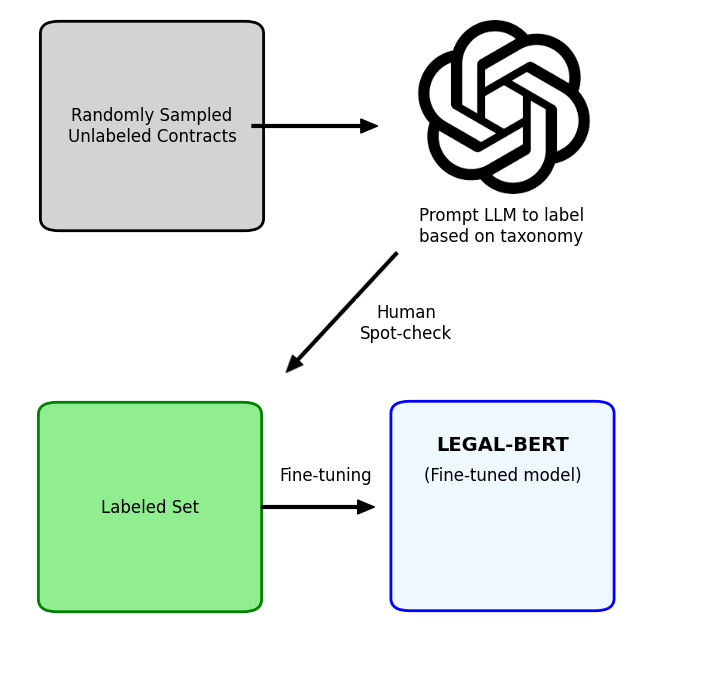
\includegraphics[width=0.6\textwidth]{llmtag.png} 
    \caption{Overview of the LLM-assisted labeling and LegalBERT training pipeline.}
    \label{fig:llm_flowchart}
\end{figure}

We first constructed a taxonomy of common legal contract types, such as Sale of Goods, Real Estate Contracts, Employment Contracts, and Licensing Agreements. Each category included clear inclusion and exclusion criteria. From a large pool of unlabeled contracts, we randomly sampled a subset (we used 5000 samples) and used GPT-4 to label them according to the taxonomy. The LLM output included predicted labels, confidence scores, and rationales. A sample of these outputs was manually reviewed to ensure accuracy.

The resulting labeled dataset was then used to fine-tune a predictive model. Prior to supervised training, we applied domain-adaptive pretraining (DAPT) by continuing masked language modeling (MLM) on the contract corpus using LegalBERT. This pretraining step used the standard cross-entropy loss over randomly masked tokens with a masking probability of 15\%. For the downstream classification task, we fine-tuned the model using weighted categorical cross-entropy, where class weights were assigned based on label frequencies to account for class imbalance, and used gradient accumulation to accommodate long sequences.

This effectively addresses the lack of labeled datasets in the legal domain by leveraging LLMs for scalable, high-quality annotation and enabling downstream training of specialized, efficient models.

\begin{table}[htbp]
\centering
\caption{Classification report on 300 testing samples}
\begin{tabular}{lcccc}
\hline
\textbf{Class} & \textbf{Precision} & \textbf{Recall} & \textbf{F1-Score} & \textbf{Support} \\
\hline
Agency Agreements & 0.3333 & 0.3333 & 0.3333 & 3 \\
Confidentiality (NDA) Agreements & 0.0000 & 0.0000 & 0.0000 & 1 \\
Construction Contracts & 1.0000 & 1.0000 & 1.0000 & 4 \\
Employment Contracts & 0.9429 & 0.7857 & 0.8571 & 42 \\
Franchise Agreements & 1.0000 & 1.0000 & 1.0000 & 1 \\
Guarantee Contracts & 0.8462 & 0.9167 & 0.8800 & 12 \\
Indemnity Contracts & 1.0000 & 0.8462 & 0.9167 & 13 \\
Insurance Contracts & 1.0000 & 0.8462 & 0.9167 & 13 \\
Lease Agreements & 0.8095 & 1.0000 & 0.8947 & 17 \\
Licensing Agreements & 0.6981 & 0.8605 & 0.7738 & 43 \\
Loan Agreements & 0.8462 & 0.9167 & 0.8800 & 24 \\
Partnership Agreements & 0.8500 & 0.7727 & 0.8095 & 22 \\
Real Estate Contracts & 1.0000 & 0.7333 & 0.8462 & 15 \\
Sale of Goods & 0.8649 & 0.9412 & 0.9014 & 34 \\
Service Contracts & 0.7027 & 0.7027 & 0.7027 & 37 \\
Settlement Agreements & 0.9091 & 0.8000 & 0.8511 & 25 \\
\hline
\textbf{Accuracy} & & & \textbf{0.8133} & 300 \\
\textbf{Macro avg} & 0.8002 & 0.7881 & 0.7902 & 300 \\
\textbf{Weighted avg} & 0.8189 & 0.8133 & 0.8113 & 300 \\
\hline
\end{tabular}
\label{tab:classification_report}
\end{table}

\subsection*{Clause Segmentation using Regex + Semantic + Supervised Bounds Detection}

To extract meaningful clause units from raw contract text, we designed a hybrid segmentation pipeline that combines rule-based, semantic, and supervised methods for clause boundary detection. This multi-pronged approach addresses the limitations of any single technique and is tailored to the variability of real-world contract formatting.

\subsubsection*{Regex-Based Boundary Detection}

Our first boundary detection step uses a suite of regular expressions to identify structural cues within contract text. These include:
\begin{itemize}
    \item Numbered section headers (e.g., \texttt{1. Definitions}, \texttt{2.1 Termination})
    \item Uppercase headers (e.g., \texttt{CONFIDENTIALITY}, \texttt{TERMINATION})
    \item Legalistic keywords such as \texttt{WHEREAS} or \texttt{NOW, THEREFORE}
\end{itemize}
These patterns are matched line-by-line to mark likely clause start points. Although effective for well-structured documents, regex alone is brittle when formatting is inconsistent or headings are missing.

\subsubsection*{Semantic Boundary Detection}

To detect shifts in meaning beyond surface patterns, we apply semantic similarity using sentence embeddings. Specifically, we use the \texttt{all-MiniLM-L6-v2} model from \texttt{SentenceTransformers} to encode each sentence in the contract into a 384-dimensional embedding. We then compute cosine similarity between adjacent sentences. A significant drop in similarity (below a threshold of 0.45) signals a potential boundary:
\begin{equation}
\text{similarity}(s_i, s_{i+1}) = \frac{s_i \cdot s_{i+1}}{\|s_i\| \|s_{i+1}\|}
\end{equation}
Sentences following sharp semantic shifts are marked as new clause beginnings. This method complements regex by identifying topic transitions not reflected in formatting.

\subsubsection*{Supervised Boundary Classification}

To further refine clause segmentation, we train a supervised classifier using a labeled dataset of clause context windows. Each instance consists of a text snippet and a binary label indicating whether a clause boundary follows. We use a pipeline with TF-IDF vectorization and logistic regression, achieving strong performance on cross-validation. This classifier captures linguistic signals missed by regex or embeddings alone, such as transitions marked by subtle discourse cues.

\subsubsection*{Boundary Merging and Clause Construction}

We combine boundary signals from all three sources—regex, semantic, and supervised—by taking the union of predicted boundary indices. The contract is then segmented into chunks based on these merged boundaries. Each resulting clause is stored with metadata including:
\begin{itemize}
    \item Clause text
    \item Detected heading (if present)
    \item Clause number (e.g., \texttt{2.1})
    \item Sentence count and position
\end{itemize}

Subclauses (e.g., \texttt{(a)}, \texttt{(b)}) are heuristically merged with their parent clauses to preserve continuity. We also apply post-filtering to discard noise (e.g., page numbers, SEC URLs) using hand-crafted rules.

\subsection*{Intra-Contract Clause Relationship Modeling}

Following segmentation, we model semantic and referential relationships between clauses within each contract. These intra-contract clause connections include:

\begin{itemize}
    \item \textbf{Term--Definition Links}: Clauses that define key terms (e.g., “Affiliate means...”) are semantically matched to clauses that contain those terms using TF-IDF-based similarity and phrase matching.
    
    \item \textbf{Cross-References}: We detect explicit references such as “See Section 4.2” using regex and link them to the corresponding clause if the section number is available.
    
    \item \textbf{Topical Clustering}: We compute pairwise semantic similarities between clauses and apply document-level clustering (e.g., DBSCAN or Agglomerative Clustering) to group clauses with similar function or legal role. This enhances contract structure analysis and redundancy detection.
\end{itemize}

These intra-clause connections are embedded as additional metadata into the clause dataset and allow downstream tasks like contextual summarization, contradiction detection, and interactive contract visualization.


\section*{Datasets}

Our project integrates both publicly available and custom-curated datasets to support clause classification, segmentation, and intra-contract analysis.

\subsection*{External Benchmarks}

We draw inspiration and structure from two widely recognized legal NLP datasets:

\begin{itemize}
    \item \textbf{CUAD (Contract Understanding Atticus Dataset)}~\cite{hendrycks2021cuad}: A dataset of 510 commercial legal contracts manually annotated by legal experts with over 13,000 clauses across 41 clause types. We reference CUAD to inform our clause taxonomy and to evaluate the strengths and limitations of general-purpose clause labeling.
    
    \item \textbf{ContractNLI}~\cite{koreeda2021contractnli}: A corpus of 607 non-disclosure agreements (NDAs) annotated for entailment, contradiction, or neutrality against 17 hypothesis statements. This dataset provided valuable insights into contract-type-specific inference and motivated our decision to specialize labels by contract domain.
\end{itemize}

\subsection*{LLM-Labeled Contract Dataset}

To overcome the lack of large-scale labeled data in the legal domain, we constructed a high-quality contract classification dataset using LLM-assisted annotation. We sampled 5,000 unlabeled legal contracts from a diverse pool and used GPT-4 to label them with one of 16 predefined contract types (e.g., Employment, Sale of Goods, Lease, Licensing). The LLM output included a predicted label, confidence score, and rationale for each instance. A random subset of outputs was manually reviewed to ensure labeling reliability.

This dataset was used to fine-tune a domain-adapted LegalBERT classifier capable of predicting contract type for unseen documents, enabling automatic integration of new contracts into our pipeline.

\subsection*{Clause Segmentation and Metadata Dataset}

Following contract classification, each contract is passed through our hybrid segmentation pipeline, yielding a clause-level dataset. Each clause unit includes the following metadata:
\begin{itemize}
    \item Contract type (from the classifier)
    \item Clause text
    \item Clause number and heading (if available)
    \item Sentence count and position
    \item Detected boundaries (regex, semantic, or supervised)

\end{itemize}

This segmented clause corpus forms the foundation for downstream tasks such as clause classification, summarization, contract fairness evaluation, and visualization. The pipeline is modular, making it possible to incrementally expand the dataset as more contracts are added.


\section*{Evaluation Results}

\textit{Describe your evaluation results. What metrics
will did you use? What baseline from an existing solutions can you compare to?}

Evalutation text here.


\section*{Conclusion}

In this project, we developed a comprehensive pipeline for legal contract analysis, focusing on clause-level segmentation, classification, and relationship modeling. Motivated by the limitations of existing datasets such as CUAD and ContractNLI, our work bridges the gap between coarse document-level tasks and fine-grained clause-level understanding.

We introduced a hybrid clause segmentation framework that merges regex-based structural cues, semantic similarity modeling using sentence embeddings, and supervised boundary detection. This approach proved effective in handling the diverse formatting and complexity of real-world contracts. For contract classification, we demonstrated how large language models such as GPT-4 can be leveraged for high-quality annotation, which enables efficient fine-tuning of smaller models like LegalBERT for scalable deployment. The classification model achieved strong performance across a diverse taxonomy of contract types.

Our framework also supports extensibility: new contracts can be seamlessly incorporated into the dataset by passing them through the classification module to assign contract type, followed by clause boundary detection to extract individual clause units, and finally intra-contract linkage modeling to capture relationships between clauses (e.g., term-definition, contextual dependencies). This modular design enables scalable dataset expansion, making it suitable for iterative annotation, downstream learning tasks, and real-world legal contract analytics.

Beyond segmentation and labeling, we explored intra-contract clause relationships, laying the groundwork for more context-aware downstream applications such as clause summarization, fairness assessment, and contract quality evaluation.

Overall, our pipeline represents a scalable and adaptable framework for clause-level contract analysis, and contributes both methodological innovations and a reproducible dataset creation process to the legal NLP community.
\begin{thebibliography}{9}

\bibitem{citation_key1}
Author1. 
\textit{Title1}.
Publisher, Year.

\bibitem{citation_key2}
Author2. 
\textit{Title2}.
Publisher, Year.

\end{thebibliography}

\end{document} 